\documentclass[xcolor=svgnames,mathserif]{beamer}
\usepackage[utf8]{inputenc}
\usepackage[T1]{fontenc}

\usepackage[english]{babel}
% pour les images
\usepackage{graphicx}
% pour les espaces entre les lignes : 1, 1.5, 2
\usepackage{setspace}
% pour les marges
\usepackage{geometry}
%infos générales du document
\usepackage{amsmath,amsfonts}
% pour les couleurs
\usepackage{color}
% pour mettre des url
\usepackage{url}
% pour les schémas
\usepackage[all]{xy}
% for bold symbols in mathmode
\usepackage{bm}
% biblio exotique
\usepackage{natbib}

\usetheme{metropolis}

% Customisation of the metropolis theme
\definecolor{deeppurple}{HTML}{29293D}
\definecolor{lightpurple}{HTML}{B3B3CC}
\definecolor{medpurple}{HTML}{666699}

\definecolor{deepblue}{HTML}{19194D}
\definecolor{medblue}{HTML}{333399}
\definecolor{lightblue}{HTML}{B3B3E6}


\definecolor{mygreen}{HTML}{3E750A}
\definecolor{mypink}{HTML}{B30047}
%% \definecolor{mypink}{HTML}{CC0052}

\setbeamercolor{normal text}{fg=deeppurple}
\setbeamercolor{frametitle}{bg=deeppurple}
\setbeamercolor{example text}{fg=mypink}
\setbeamercolor{accent text}{fg=myblue}
\setbeamercolor{alerted text}{fg=mypink}
\setbeamercolor{progress bar}{fg=mypink}

\metroset{sectionpage=progressbar, subsectionpage=none, progressbar=frametitle}


\newcommand{\R}{\mathbb{R}}
\newcommand{\beq}{\begin{equation}}
\newcommand{\eeq}{\end{equation}}
\newcommand{\m}[1]{\mathbf{#1}}
\newcommand{\Rlogo}{
\includegraphics[width=0.05\textwidth]{figs/Rlogo-transp}~}


\title[R Epidemics Consortium]{
\includegraphics[width=.4\textwidth]{figs/recon-logo.png}}

\subtitle{Building the next generation of statistical tools for outbreak response using R}

\author[T. Jombart]{Thibaut Jombart}

\institute{Imperial College London\\MRC Centre for Outbreak Analysis and Modelling}
\date{18th April 2017}




\begin{document}




%%%%%%%%%%%%%%%%%%%%%%%%%%%%
%%%%%%%%%%%%%%%%%%%%%%%%%%%%
\begin{frame}[fragile]
  \frametitle{~}
  \vspace{-.3cm}

  \titlepage
\end{frame}
%%%%%%%%%%%%%%%%%%%%%%%%%%%%
%%%%%%%%%%%%%%%%%%%%%%%%%%%%






%%%%%%%%%%%%%%%%%%%%%%%%%%%%
%%%%%%%%%%%%%%%%%%%%%%%%%%%%
\begin{frame}{Outline}
  \setbeamertemplate{section in toc}[sections numbered]
  \tableofcontents[hideallsubsections]
\end{frame}
%%%%%%%%%%%%%%%%%%%%%%%%%%%%
%%%%%%%%%%%%%%%%%%%%%%%%%%%%






%%%%%%%%%%%%%%%%%%%%%%%%%%%%
%%%%%%%%%%%%%%%%%%%%%%%%%%%%
\section[Ebola response]{Lessons learnt from the Ebola outbreak response}
%%%%%%%%%%%%%%%%%%%%%%%%%%%%
%%%%%%%%%%%%%%%%%%%%%%%%%%%%



%%%%%%%%%%%%%%%%%%%%%%%%%%%%
%%%%%%%%%%%%%%%%%%%%%%%%%%%%
\begin{frame}[fragile]
  \frametitle{Lessons learnt from the Ebola response}

\vspace{-2cm}
\begin{center} 

\only<1>{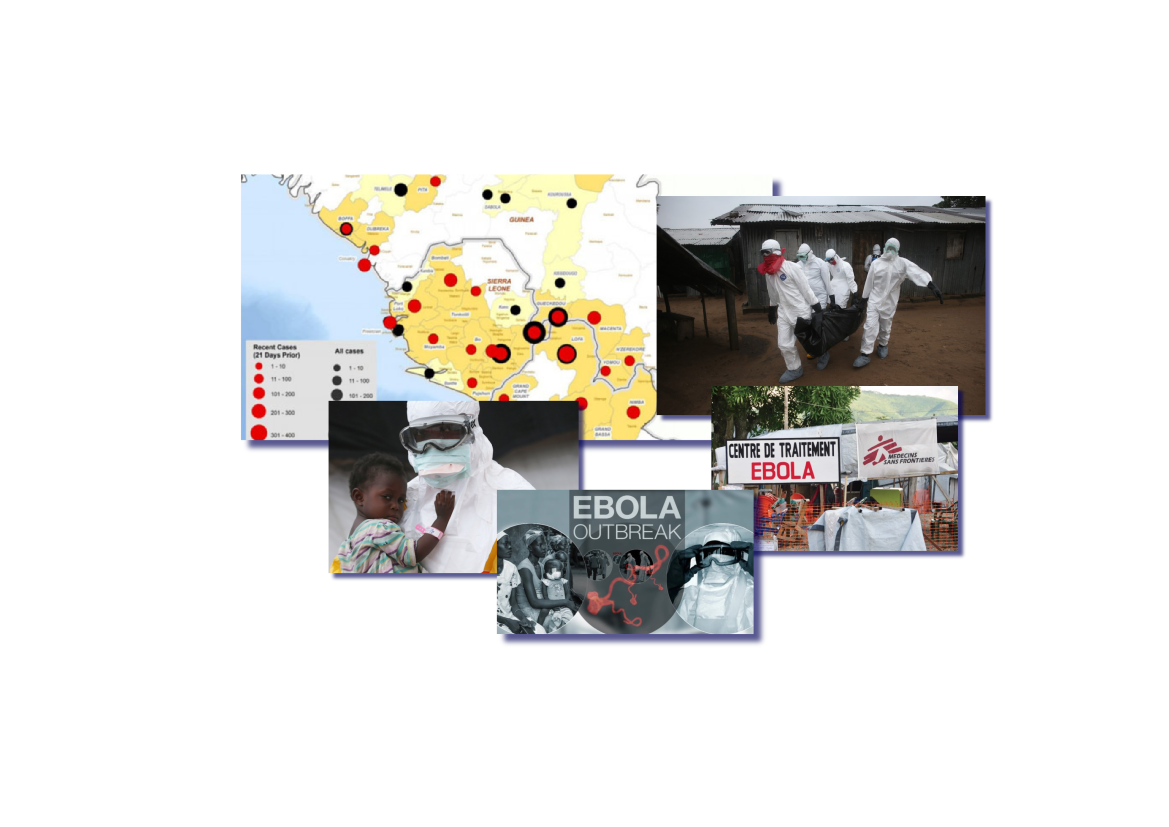
\includegraphics[width=.9\textwidth]{figs/motivation1}}\only<2>{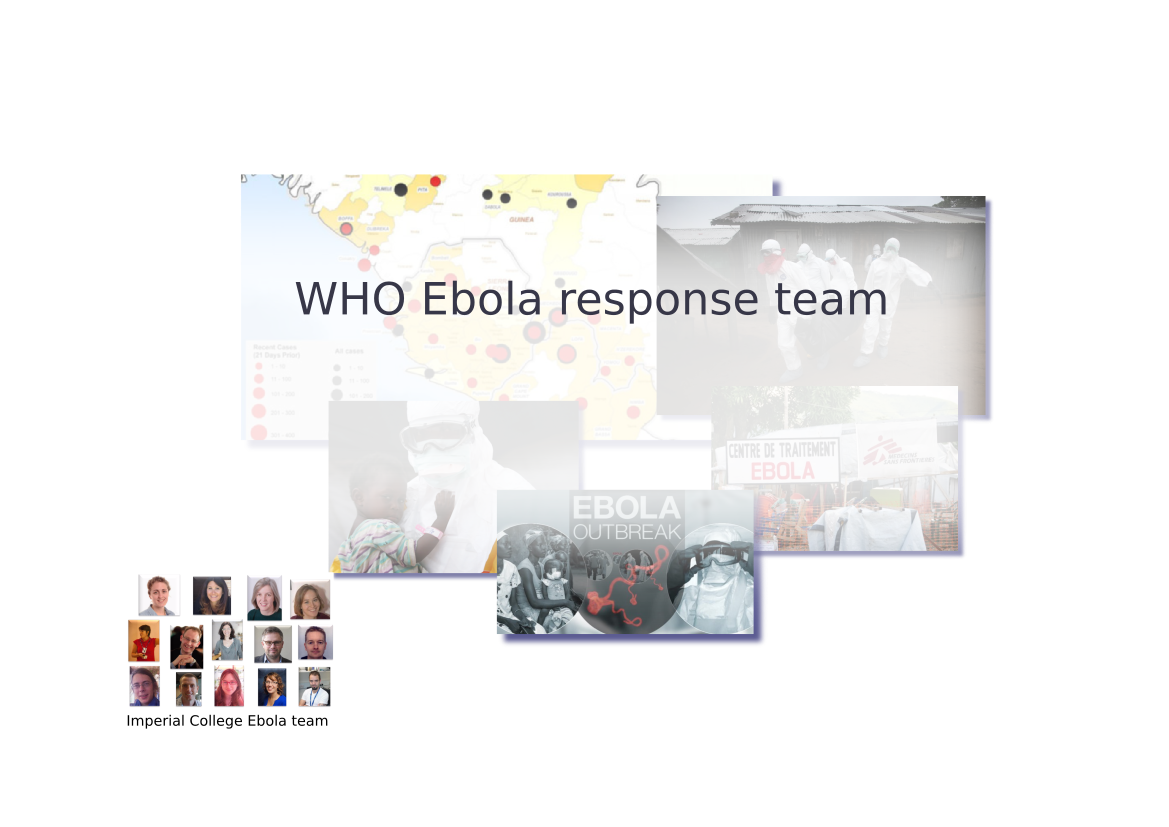
\includegraphics[width=.9\textwidth]{figs/motivation2}}\only<3->{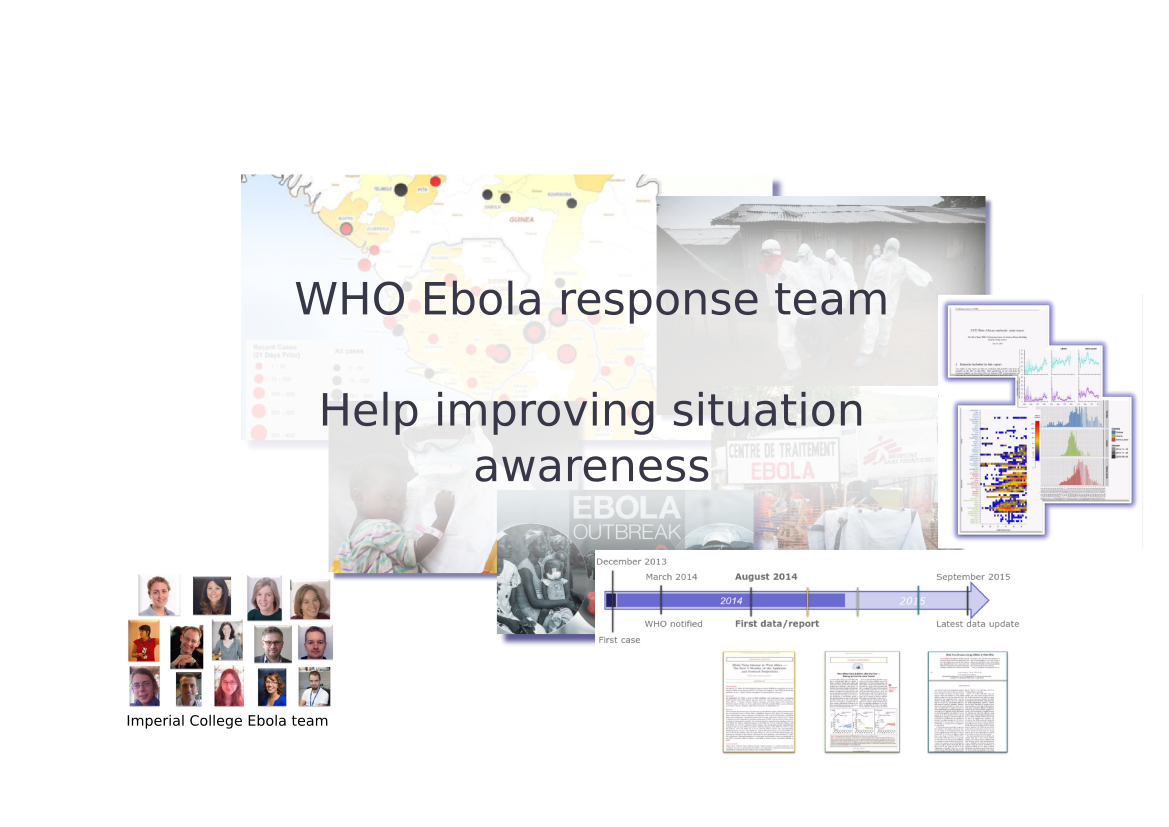
\includegraphics[width=.9\textwidth]{figs/motivation3}}


\visible<4>{\emph{Most statistical/modelling tools for situation awareness missing.}}

\end{center}


\end{frame}
%%%%%%%%%%%%%%%%%%%%%%%%%%%%
%%%%%%%%%%%%%%%%%%%%%%%%%%%%





%%%%%%%%%%%%%%%%%%%%%%%%%%%%
%%%%%%%%%%%%%%%%%%%%%%%%%%%%
\begin{frame}[fragile]
  \frametitle{What tools do we need?}

  Some examples: 
  
  \begin{itemize}
   \item \textbf{data cleaning:} dictionaries, entry matching
%    \pause 
   \vspace{.3cm}
   \item \textbf{graphics:} case incidence in space and time, contact tracing
%    \pause 
   \vspace{.3cm}
   \item \textbf{parameter estimation:} key delays, transmissibility
%    \pause
   \vspace{.3cm}
   \item \textbf{estimate / test CFR:} gender, health care workers, treaments effects
%    \pause
   \vspace{.3cm}
   \item \textbf{predictions:} case incidence, mortality, evaluate interventions
%    \pause 
   \vspace{.3cm}
   \item \textbf{report:} (semi-)automated situation reports
%    \pause \vspace{.3cm}
%    \item \textbf{and more!}
  \end{itemize}


\end{frame}
%%%%%%%%%%%%%%%%%%%%%%%%%%%%
%%%%%%%%%%%%%%%%%%%%%%%%%%%%






%%%%%%%%%%%%%%%%%%%%%%%%%%%%
%%%%%%%%%%%%%%%%%%%%%%%%%%%%
\begin{frame}[fragile]
  \frametitle{Who do we need to develop these tools?}

\vspace{-.5cm}
\begin{center} 

\only<1>{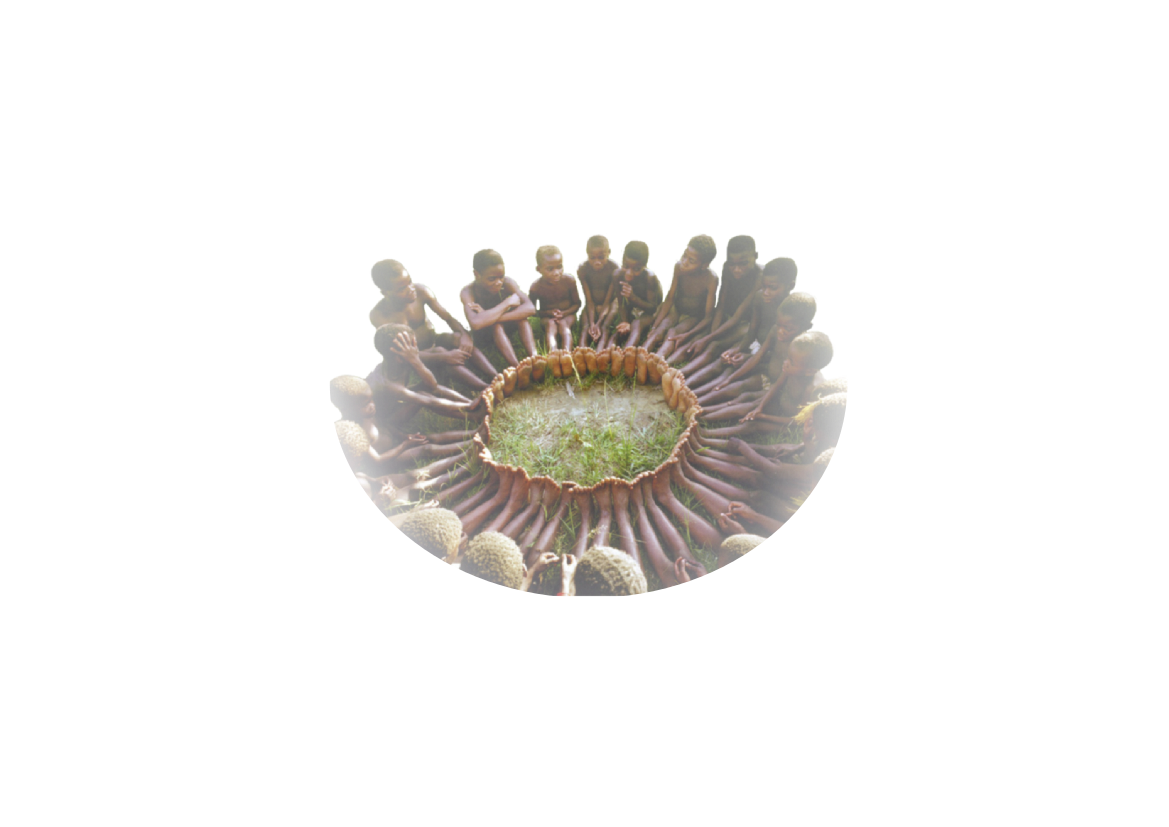
\includegraphics[width=.8\textwidth]{figs/worlds1}}\only<2>{
\includegraphics[width=.8\textwidth]{figs/worlds2}}\only<3>{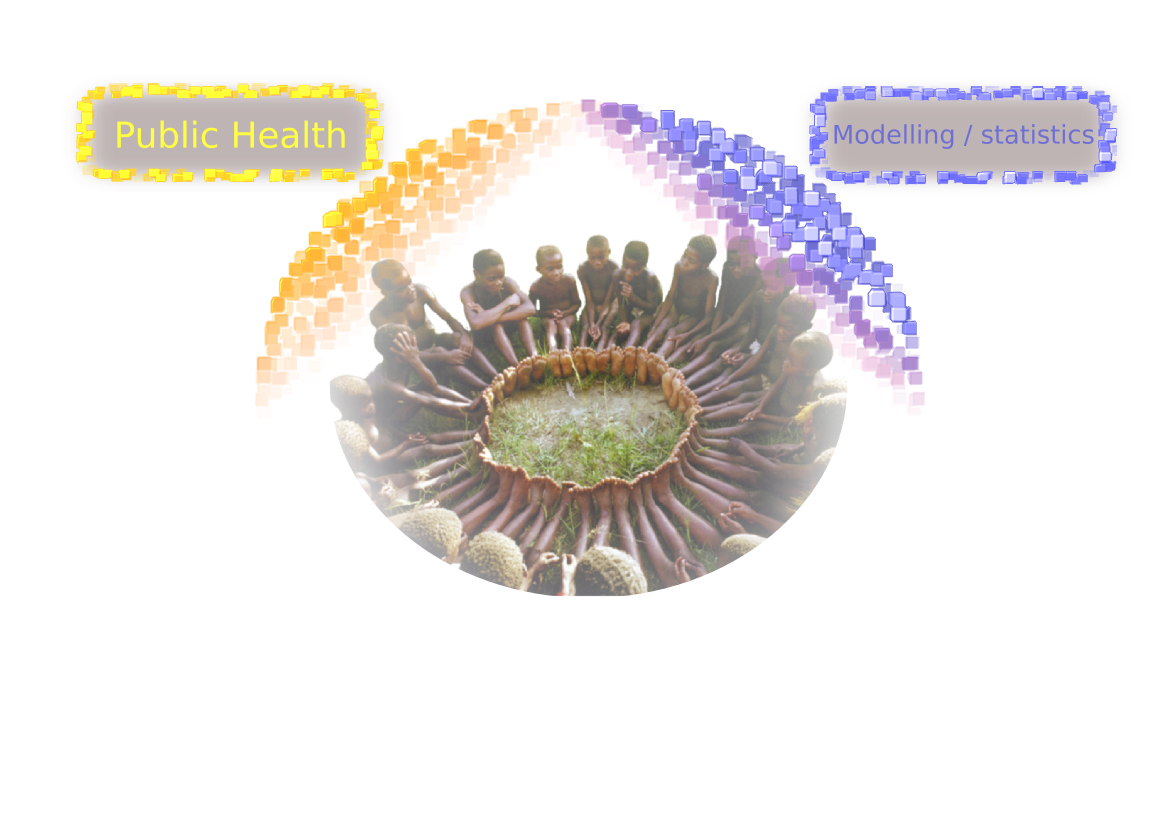
\includegraphics[width=.8\textwidth]{figs/worlds3}}\only<4->{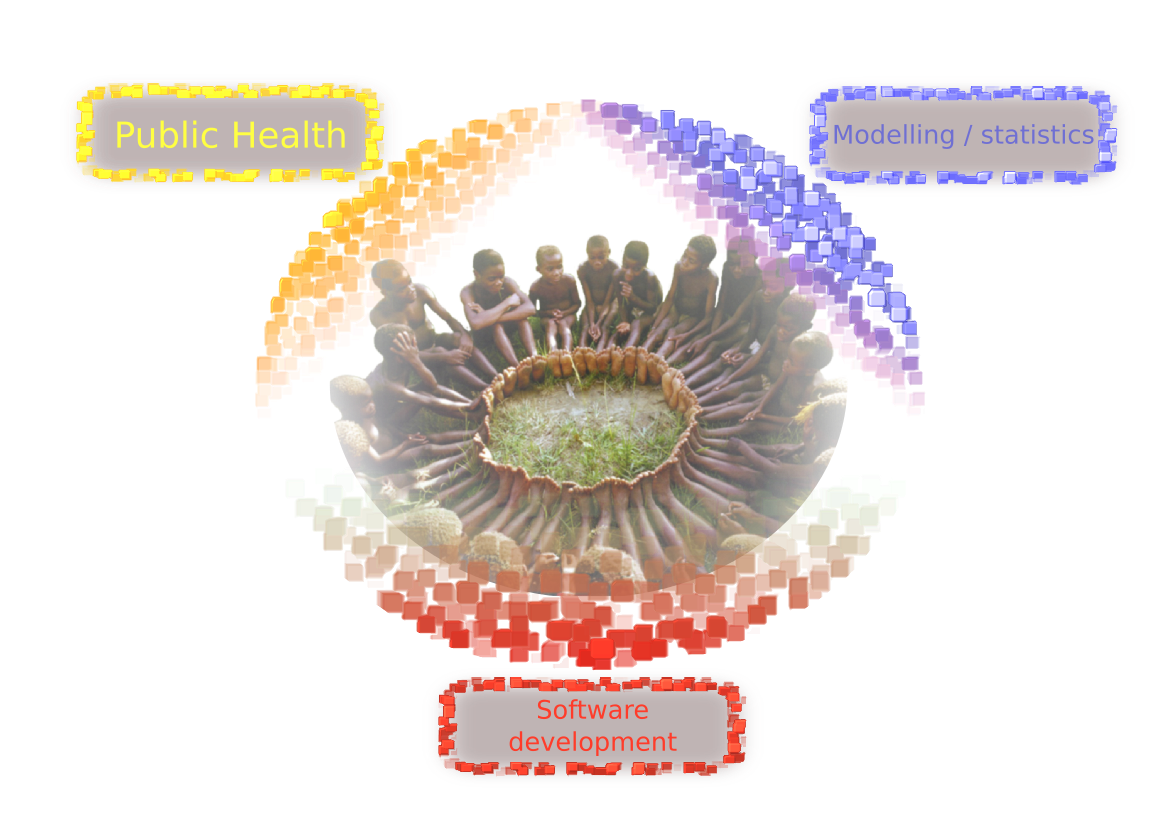
\includegraphics[width=.8\textwidth]{figs/worlds4}}

\end{center}


\end{frame}
%%%%%%%%%%%%%%%%%%%%%%%%%%%%
%%%%%%%%%%%%%%%%%%%%%%%%%%%%






%%%%%%%%%%%%%%%%%%%%%%%%%%%%
%%%%%%%%%%%%%%%%%%%%%%%%%%%%
\section{The R Epidemics Consortium}
%%%%%%%%%%%%%%%%%%%%%%%%%%%%
%%%%%%%%%%%%%%%%%%%%%%%%%%%%


%%%%%%%%%%%%%%%%%%%%%%%%%%%%
%%%%%%%%%%%%%%%%%%%%%%%%%%%%
\begin{frame}[fragile]
  \frametitle{Hackout 3: a \Rlogo hackathon for emergency outbreak response}

  Last summer at the \textit{rOpenSci} headquarters (Berkeley)
\vspace{-.3cm}
\begin{center} 

\includegraphics[width=.75 \textwidth]{figs/hackout3}
\end{center}


\end{frame}
%%%%%%%%%%%%%%%%%%%%%%%%%%%%
%%%%%%%%%%%%%%%%%%%%%%%%%%%%






%%%%%%%%%%%%%%%%%%%%%%%%%%%%
%%%%%%%%%%%%%%%%%%%%%%%%%%%%
\begin{frame}[fragile]
  \frametitle{Hackout 3: from ideas to projects to...}

\vspace{-.3cm}
\begin{center} 
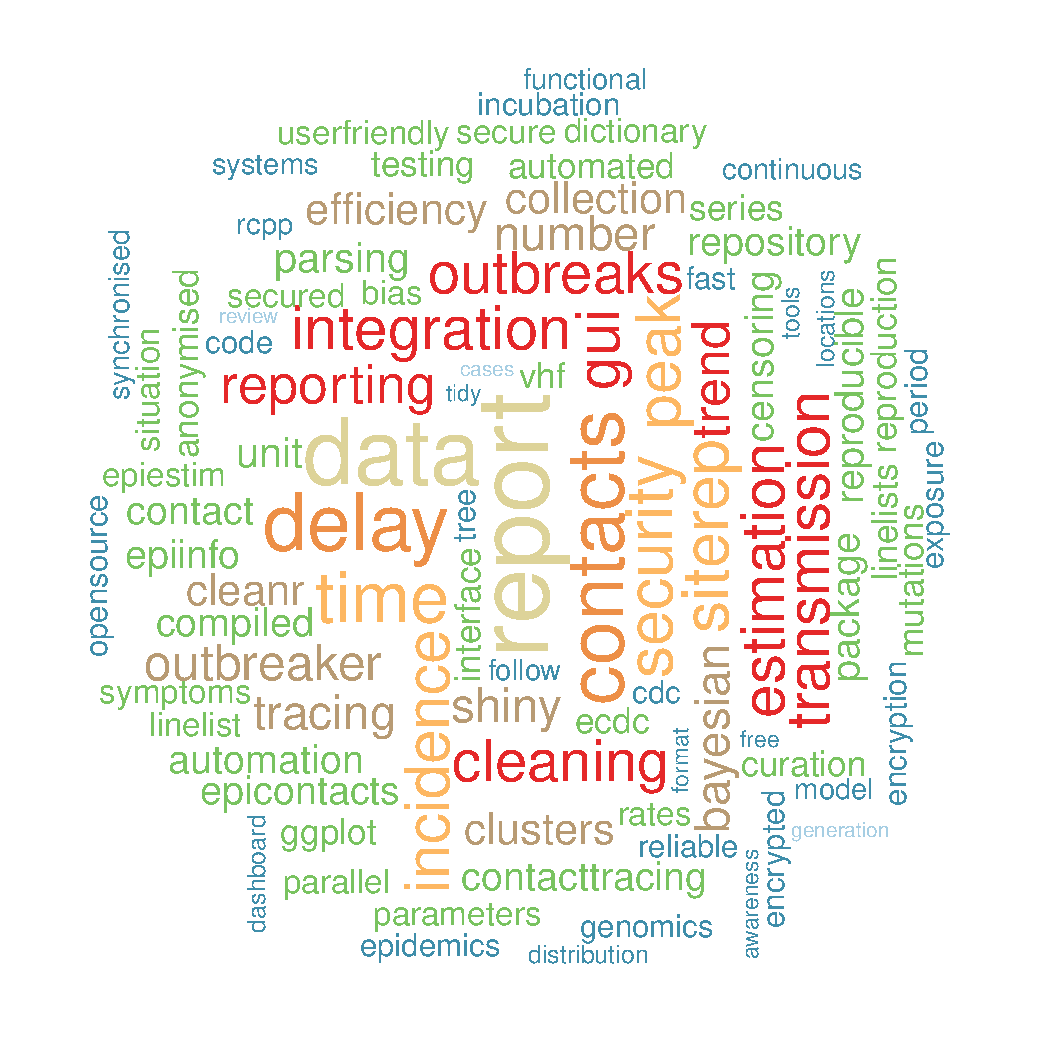
\includegraphics[width=.65 \textwidth]{figs/wordcloud.pdf}

\pause
\emph{How do we keep momentum once the event is over?}
\end{center}


\end{frame}
%%%%%%%%%%%%%%%%%%%%%%%%%%%%
%%%%%%%%%%%%%%%%%%%%%%%%%%%%






%%%%%%%%%%%%%%%%%%%%%%%%%%%%
%%%%%%%%%%%%%%%%%%%%%%%%%%%%
\begin{frame}[fragile]
  \frametitle{RECON: the \textbf{R} \textbf{E}pidemics \textbf{Con}sortium}
  
  %% \vspace{-.2cm}
\small A taskforce to build a new generation of outbreak response tools in \Rlogo.

%  \vspace{-.3cm}
\begin{center} 

\includegraphics[width=.75 \textwidth]{figs/recon}
~\\
{\tiny \emph{\url{www.repidemicsconsortium.org}}}
\end{center}


\end{frame}
%%%%%%%%%%%%%%%%%%%%%%%%%%%%
%%%%%%%%%%%%%%%%%%%%%%%%%%%%






%%%%%%%%%%%%%%%%%%%%%%%%%%%%
%%%%%%%%%%%%%%%%%%%%%%%%%%%%
\begin{frame}[fragile]
  \frametitle{In a nutshell}

  
\includegraphics[width=.5 \textwidth]{figs/recon-logo}
  ~\\
  \emph{\url{www.repidemicsconsortium.org}}

  \begin{itemize}
    
  \item started 6th September 2016 
    %   \pause
    \vspace{.2cm}
  \item 60 people (54 members, 6 board)
    %   \pause
    \vspace{.2cm}
  \item 14 countries, $>$ 30 institutions
    %   \pause
    \vspace{.2cm}
  \item 2 new packages released, $\sim$ 10-15 in development
    %   \pause
    \vspace{.2cm}
  \item involvement in training programmes starting in 2017 (FETP, EPIET, ...)
    \vspace{.2cm}
  \item \alert{public forum}, blog, online resources
  \end{itemize}

\end{frame}
%%%%%%%%%%%%%%%%%%%%%%%%%%%%
%%%%%%%%%%%%%%%%%%%%%%%%%%%%





%%%%%%%%%%%%%%%%%%%%%%%%%%%%
%%%%%%%%%%%%%%%%%%%%%%%%%%%%
\begin{frame}[fragile]
  \frametitle{The RECON forum}

\begin{center}
A platform for discussing epidemics analysis in \Rlogo.

  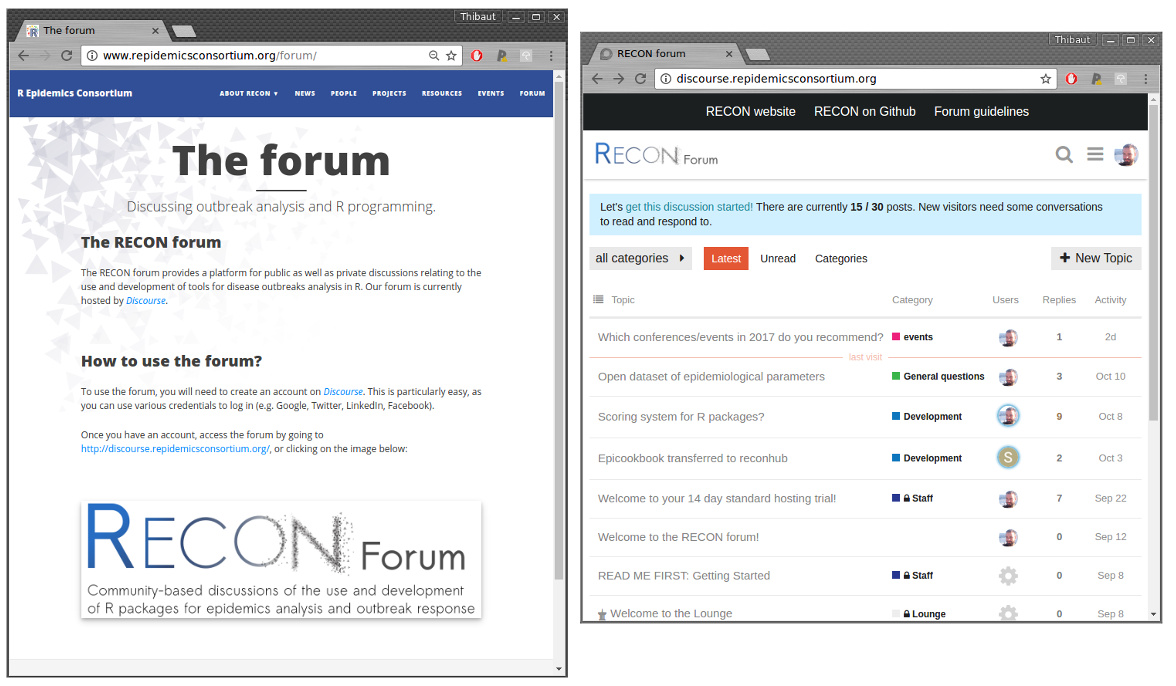
\includegraphics[width=.9\textwidth]{figs/forum}\\
\vspace{-.35cm}
{\tiny \emph{\url{www.repidemicsconsortium.org/forum}}}
\pause
~\\
\huge{\alert{Join us!}}

\end{center}


\end{frame}
%%%%%%%%%%%%%%%%%%%%%%%%%%%%
%%%%%%%%%%%%%%%%%%%%%%%%%%%%






%%%%%%%%%%%%%%%%%%%%%%%%%%%%
%%%%%%%%%%%%%%%%%%%%%%%%%%%%
\begin{frame}[fragile]
  \frametitle{RECON package: what do we aim for?}

 \begin{itemize} 
 \item \textbf{efficiency}: useful for improving situation awareness in real time; \alert{cutting-edge, computer-efficient statistical methods}
  \pause
 \vspace{.2cm}
 \item \textbf{reliability}: outputs can be trusted; \alert{continuous integration, extensive unit testing, code review, good practices}
  \pause
 \vspace{.2cm}
 \item \textbf{accessibility}: widely available, easy learning curve; \alert{extensive documentation, tutorials, websites, forum}
 \end{itemize}


\end{frame}
%%%%%%%%%%%%%%%%%%%%%%%%%%%%
%%%%%%%%%%%%%%%%%%%%%%%%%%%%









%%%%%%%%%%%%%%%%%%%%%%%%%%%%
%%%%%%%%%%%%%%%%%%%%%%%%%%%%
\section{Up-and-coming RECON packages}
%%%%%%%%%%%%%%%%%%%%%%%%%%%%
%%%%%%%%%%%%%%%%%%%%%%%%%%%%


%%%%%%%%%%%%%%%%%%%%%%%%%%%%
%%%%%%%%%%%%%%%%%%%%%%%%%%%%
\begin{frame}[fragile]
  \frametitle{\textit{incidence}: computation, handling, visualisation and modelling of epicurves}

\begin{center} 

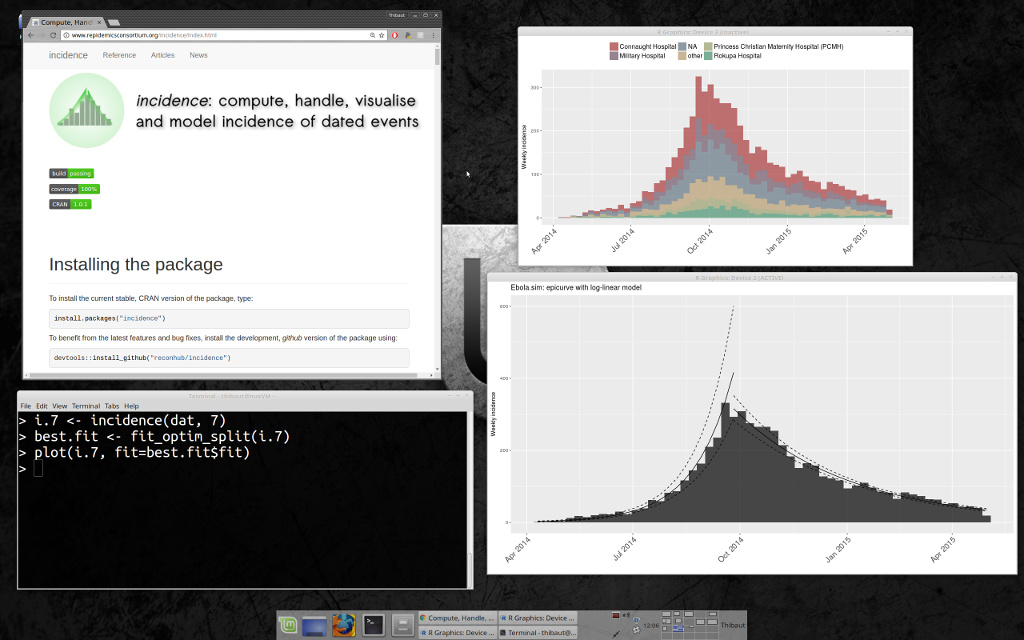
\includegraphics[width=.95\textwidth]{figs/incidence-demo}
~\\
{\scriptsize\emph{\url{www.repidemicsconsortium.org/incidence}}\\
$[$\alert{released}$]$}
}
  
\end{center}

\end{frame}
%%%%%%%%%%%%%%%%%%%%%%%%%%%%
%%%%%%%%%%%%%%%%%%%%%%%%%%%%






%%%%%%%%%%%%%%%%%%%%%%%%%%%%
%%%%%%%%%%%%%%%%%%%%%%%%%%%%
\begin{frame}[fragile]
  \frametitle{\textit{epicontacts}: handling, visualisation and analysis of epidemiological contacts}


\begin{center} 

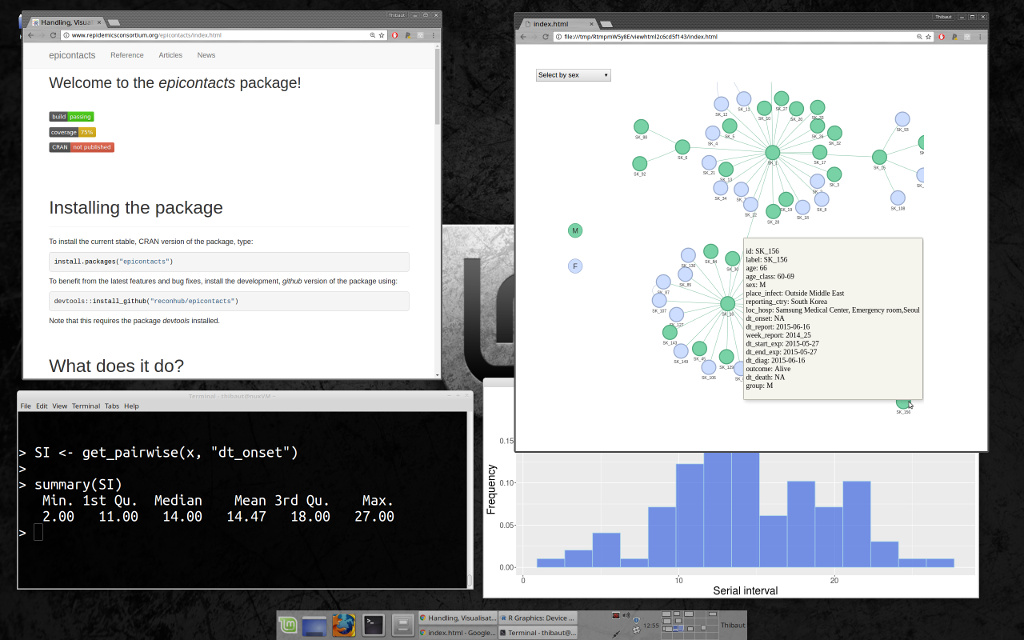
\includegraphics[width=.95\textwidth]{figs/epicontacts-demo}
~\\
{\scriptsize\emph{\url{www.repidemicsconsortium.org/epicontacts}}\\
  {\scriptsize $[$\alert{release May 2017}$]$}
}

\end{center}


\end{frame}
%%%%%%%%%%%%%%%%%%%%%%%%%%%%
%%%%%%%%%%%%%%%%%%%%%%%%%%%%





%%%%%%%%%%%%%%%%%%%%%%%%%%%%
%%%%%%%%%%%%%%%%%%%%%%%%%%%%
\begin{frame}[fragile]
  \frametitle{\textit{outbreaker2}: inferring who infects whom in an outbreak}

Original \textit{outbreaker} model: timing of symptoms and pathogen genomes to infer infectors
\\{\tiny (Jombart \textit{et al}, PLoS Comp Biol, 2014)}

\begin{center}
\only<1>{\resizebox{0.55\textwidth}{!}{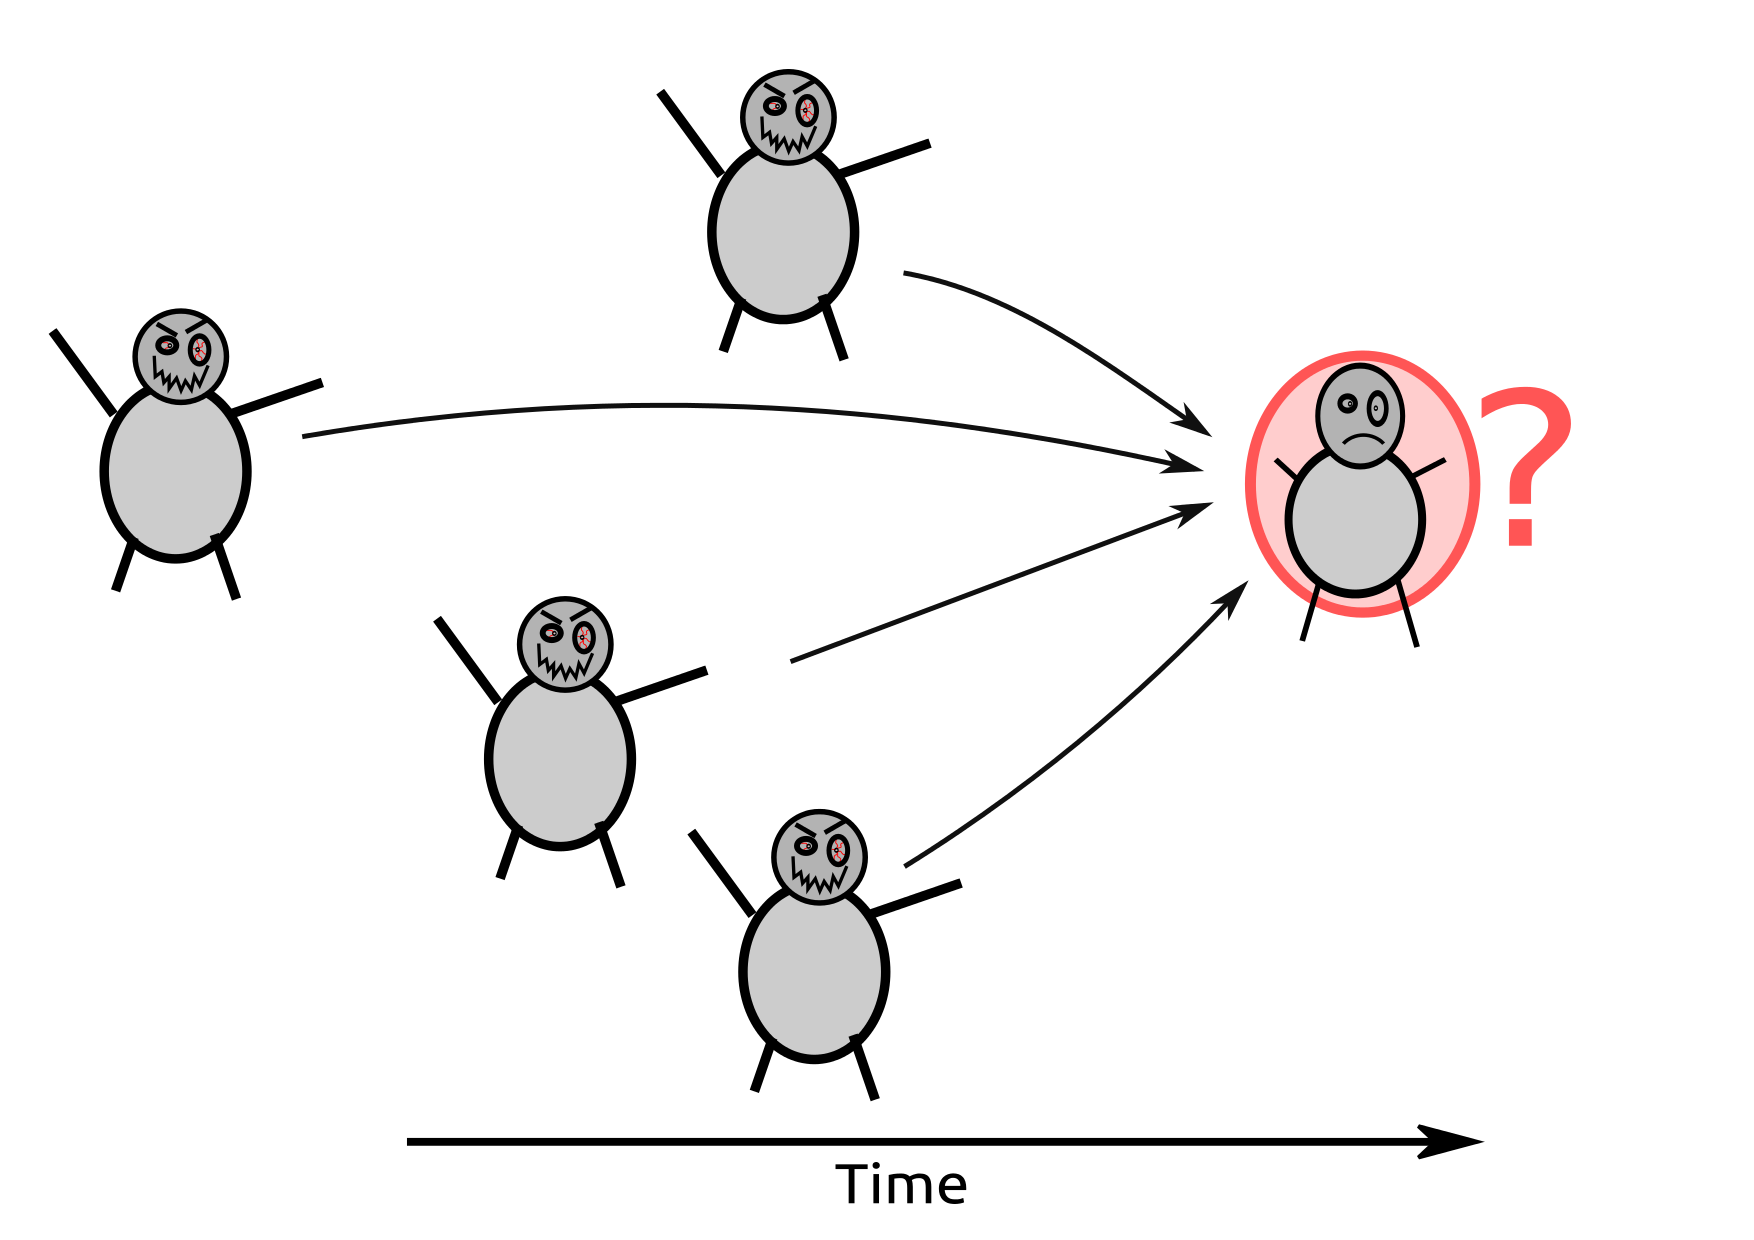
\includegraphics{figs/outbreaker-idea1}}}\only<2>{\resizebox{0.55\textwidth}{!}{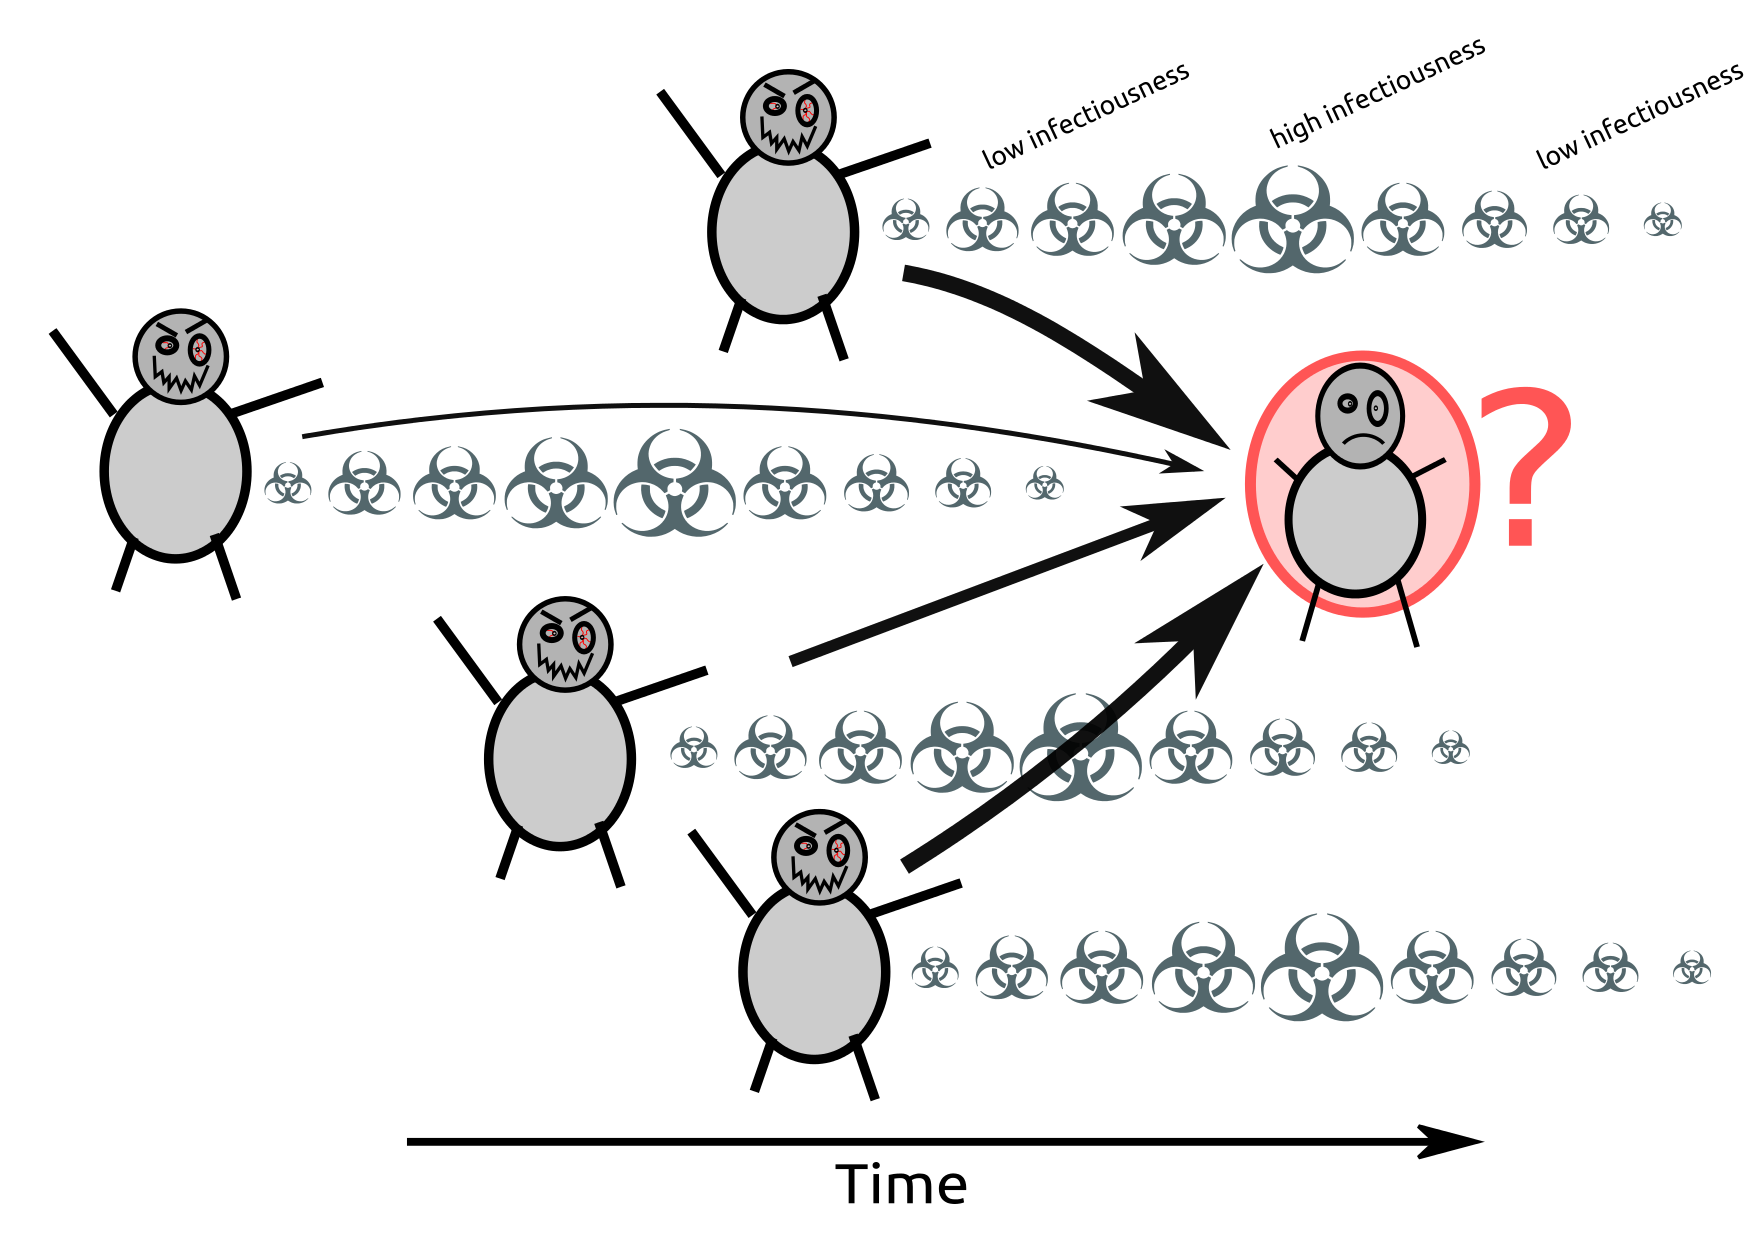
\includegraphics{figs/outbreaker-idea2}}}\only<3->{\resizebox{0.55\textwidth}{!}{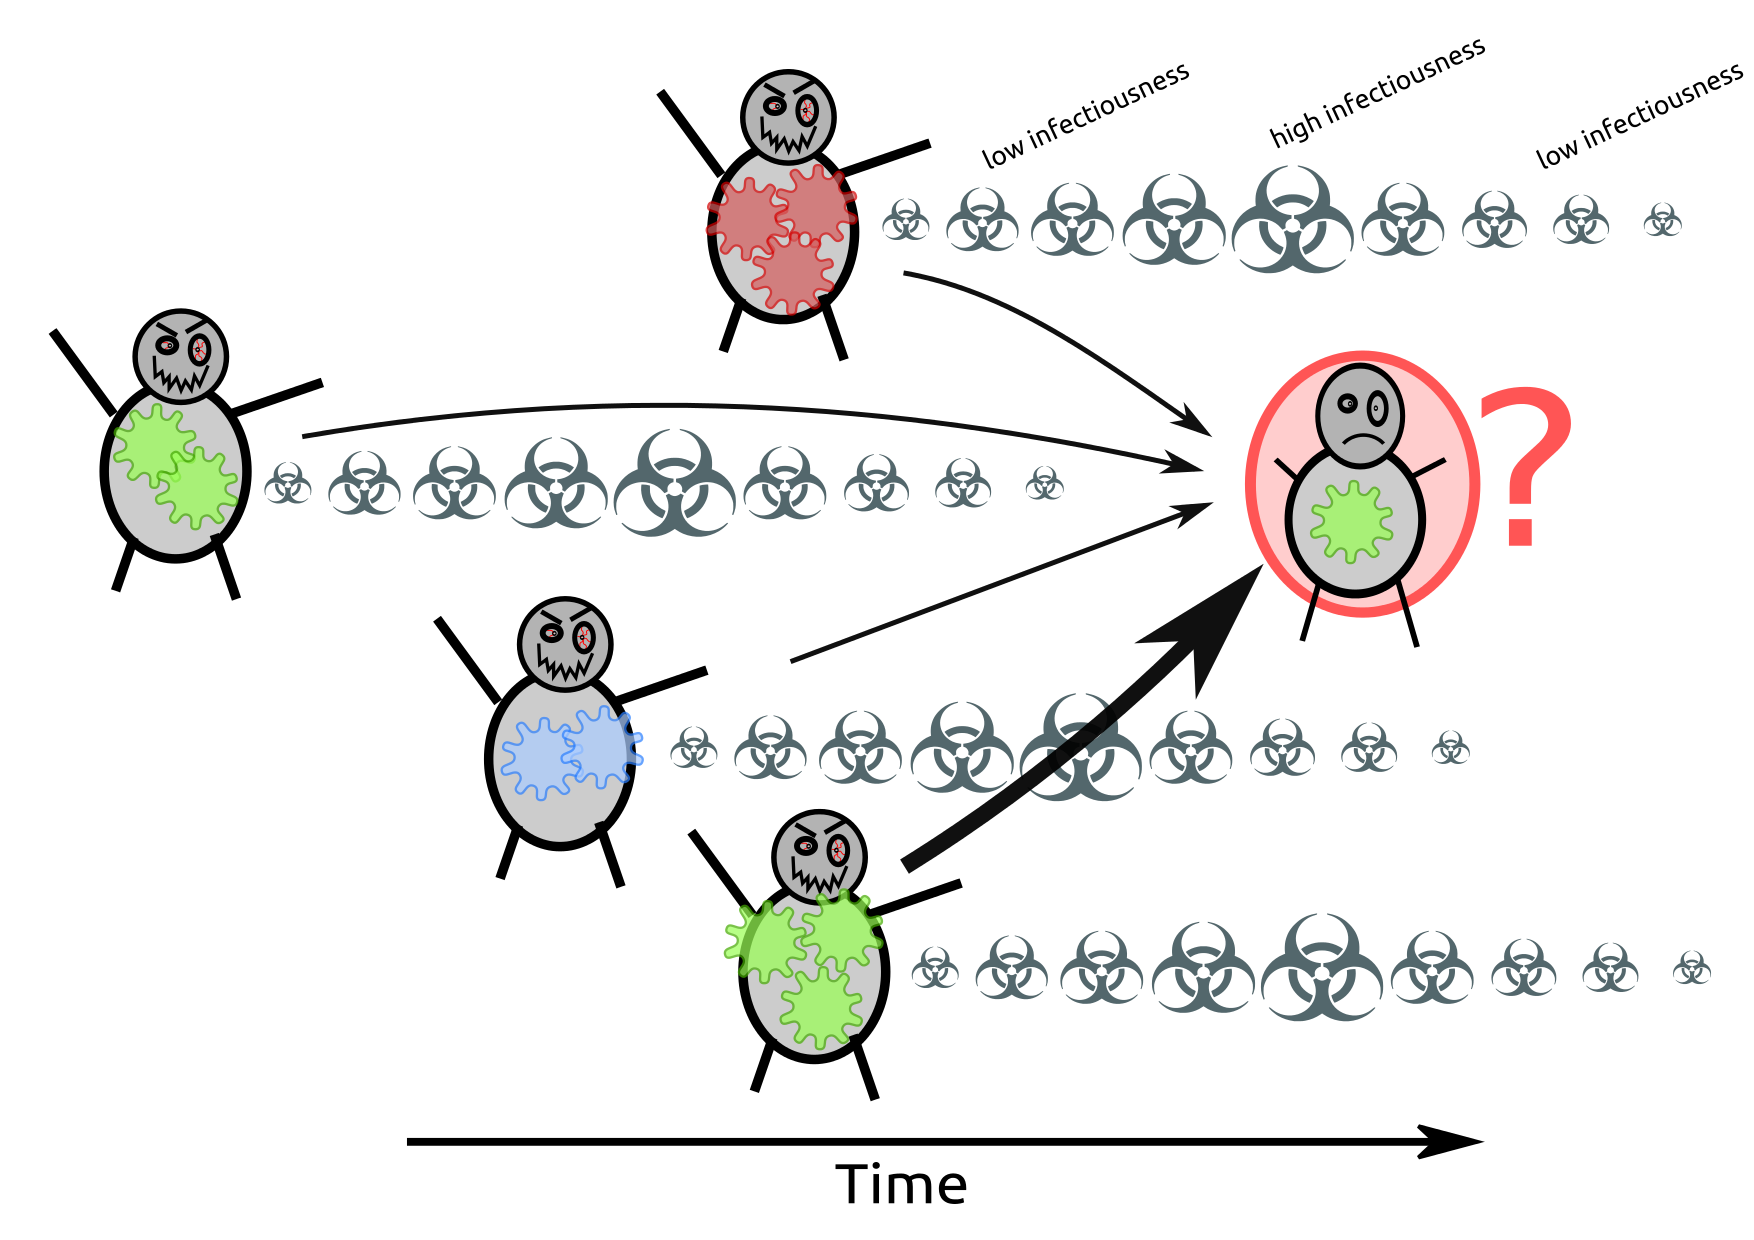
\includegraphics{figs/outbreaker-idea3}}}


\pause
%% \vspace{.5cm}
 Since \textit{outbreaker}: new models, data, and questions.
\pause
~\\
\textbf{\alert{But:} methodological niche fragmented.}
\end{center}

\end{frame}
%%%%%%%%%%%%%%%%%%%%%%%%%%%%
%%%%%%%%%%%%%%%%%%%%%%%%%%%%





%%%%%%%%%%%%%%%%%%%%%%%%%%%%
%%%%%%%%%%%%%%%%%%%%%%%%%%%%
\begin{frame}[fragile]
  \frametitle{Are different methods really... different?}

\begin{center}

  \pause
  
\includegraphics[width=.6\textwidth]{figs/wheel}
    
  \pause
  Different models can lead to very similar implementations.\\
  Can we find a \alert{general formulation}?

\end{center}

\end{frame}
%%%%%%%%%%%%%%%%%%%%%%%%%%%%
%%%%%%%%%%%%%%%%%%%%%%%%%%%%





%%%%%%%%%%%%%%%%%%%%%%%%%%%%
%%%%%%%%%%%%%%%%%%%%%%%%%%%%
\begin{frame}[fragile]
  \frametitle{What do these model look like?}

\begin{itemize}
\item $a,b,c$: different types of data
\item $\theta$: parameters / augmented data
\end{itemize}

Data are often assumed to be \emph{conditionally independent}:
$$
p(a,b,c | \theta) = p(a|\theta) p(b|\theta) p(c|\theta) 
$$
\pause
Components can be treated as \alert{plugins}.

\end{frame}
%%%%%%%%%%%%%%%%%%%%%%%%%%%%
%%%%%%%%%%%%%%%%%%%%%%%%%%%%






%%%%%%%%%%%%%%%%%%%%%%%%%%%%
%%%%%%%%%%%%%%%%%%%%%%%%%%%%
\begin{frame}[fragile]
  \frametitle{\textit{outbreaker2}: a general cauldron for cooking methods}
% \vspace{-.5cm}

Use-your-own: data type, likelihood, prior, MCMC.

\begin{center}
\only<1>{\resizebox{0.85\textwidth}{!}{\includegraphics{figs/outbreaker2idea1}}}\only<2>{\resizebox{0.85\textwidth}{!}{\includegraphics{figs/outbreaker2idea2}}}\only<3->{\resizebox{0.85\textwidth}{!}{\includegraphics{figs/outbreaker2idea3}}}

\vspace{-.25cm}
\visible<4->{\alert{Modularity} is key to generalising approaches}
\end{center}


\end{frame}
%%%%%%%%%%%%%%%%%%%%%%%%%%%%
%%%%%%%%%%%%%%%%%%%%%%%%%%%%





%%%%%%%%%%%%%%%%%%%%%%%%%%%%
%%%%%%%%%%%%%%%%%%%%%%%%%%%%
\begin{frame}[fragile]
  \frametitle{\textit{outbreaker2}: a general tool for outbreak reconstruction}
  
\begin{columns}[c c]
  \column{0.4\textwidth}
  
\begin{center}
\only<1-5>{\resizebox{1.3\textwidth}{!}{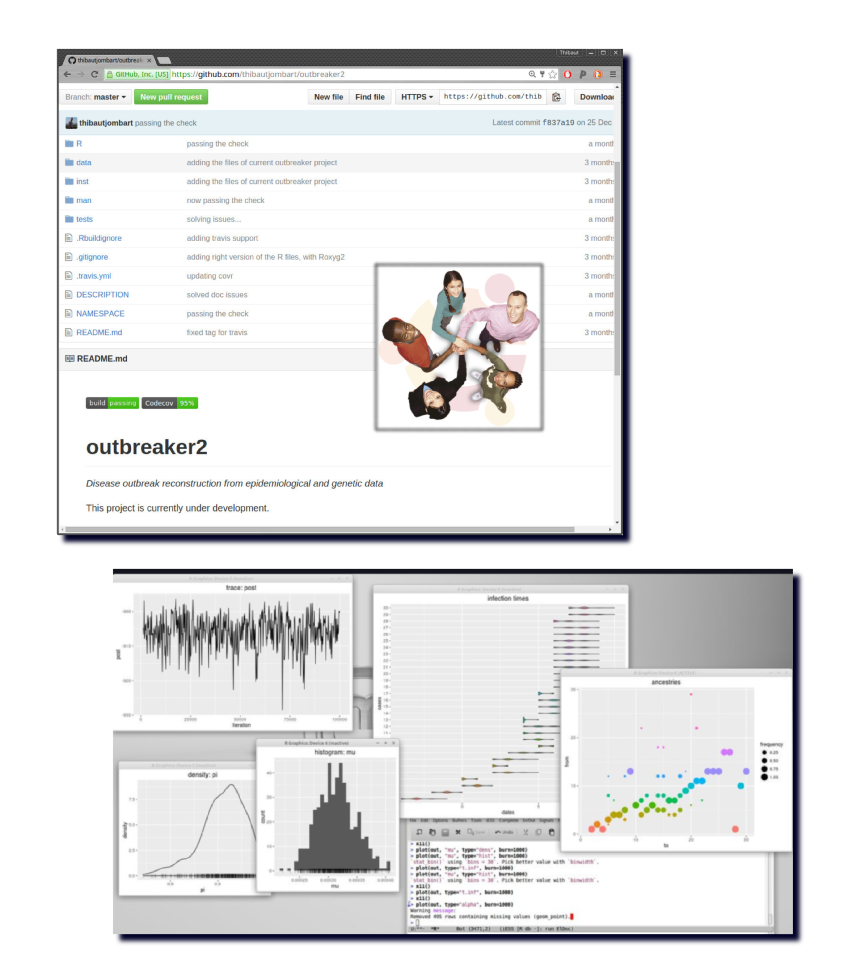
\includegraphics{figs/outbreaker2status}}}%\only<6->{\resizebox{1.3\textwidth}{!}{\includegraphics{figs/outbreaker2status2}}}
\end{center}

\pause
  \column{0.6\textwidth}

  \small
%% \begin{block}{Objectives}
\begin{itemize}
\item \textbf{modularity}: likelihood, priors, samplers are all modules\pause
\item \textbf{new 'extensions'}: contact tracing, spatial structure, new MCMC\pause
\item \textbf{reliability}: continuous integration, extensive unit testing (aiming for 100\% coverage)\pause
\item \textbf{prettier}: plot methods using \textit{ggplot2}, interactive networks visualisation\pause
\item should \alert{facilitate new contributions}
\end{itemize}
%% \end{block}

\end{columns}


\end{frame}
%%%%%%%%%%%%%%%%%%%%%%%%%%%%
%%%%%%%%%%%%%%%%%%%%%%%%%%%%







%%%%%%%%%%%%%%%%%%%%%%%%%%%%
%%%%%%%%%%%%%%%%%%%%%%%%%%%%
\section[Methodological dialogue]{Methodological dialogue during outbreak response}
%%%%%%%%%%%%%%%%%%%%%%%%%%%%
%%%%%%%%%%%%%%%%%%%%%%%%%%%%


%%%%%%%%%%%%%%%%%%%%%%%%%%%%
%%%%%%%%%%%%%%%%%%%%%%%%%%%%
\begin{frame}[fragile]
  \frametitle{Methodological development relies on an interdisciplinary dialogue}
  
  \begin{center} 

\only<1>{
\includegraphics[width=.8\textwidth]{figs/dialogue1}}\only<2>{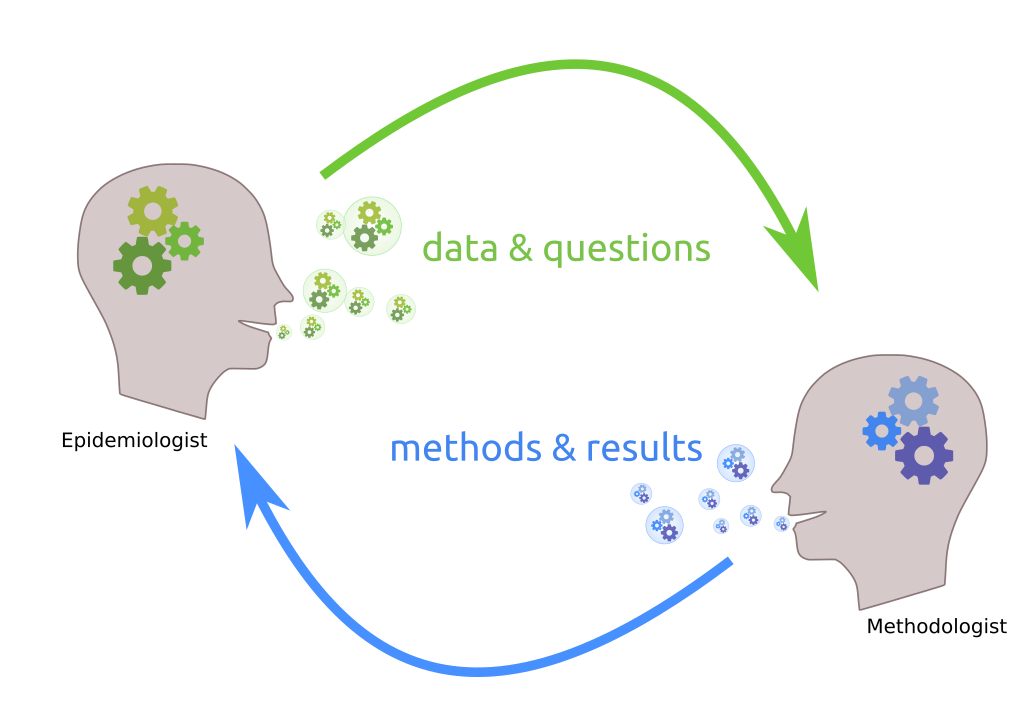
\includegraphics[width=.8\textwidth]{figs/dialogue2}}\only<3>{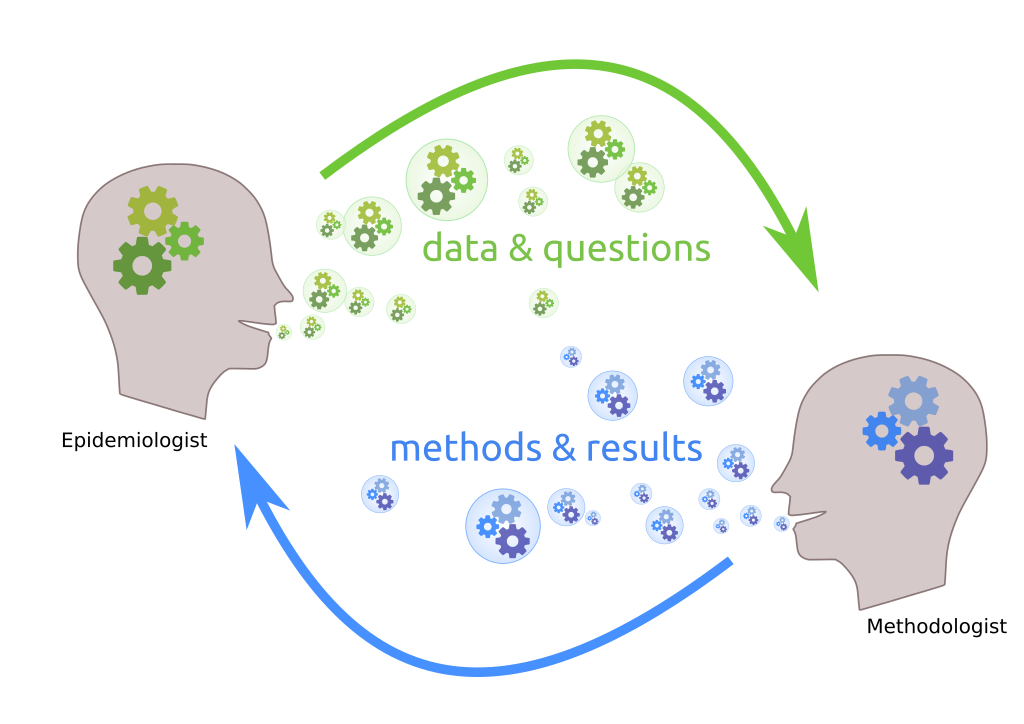
\includegraphics[width=.8\textwidth]{figs/dialogue3}}\only<4>{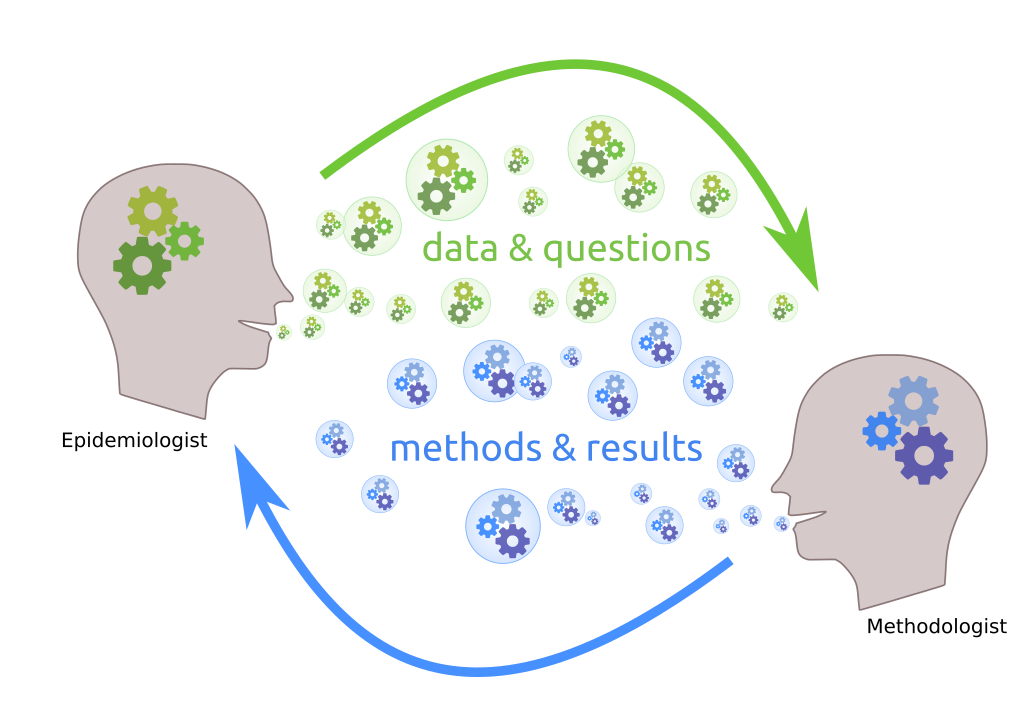
\includegraphics[width=.8\textwidth]{figs/dialogue4}}\only<5->{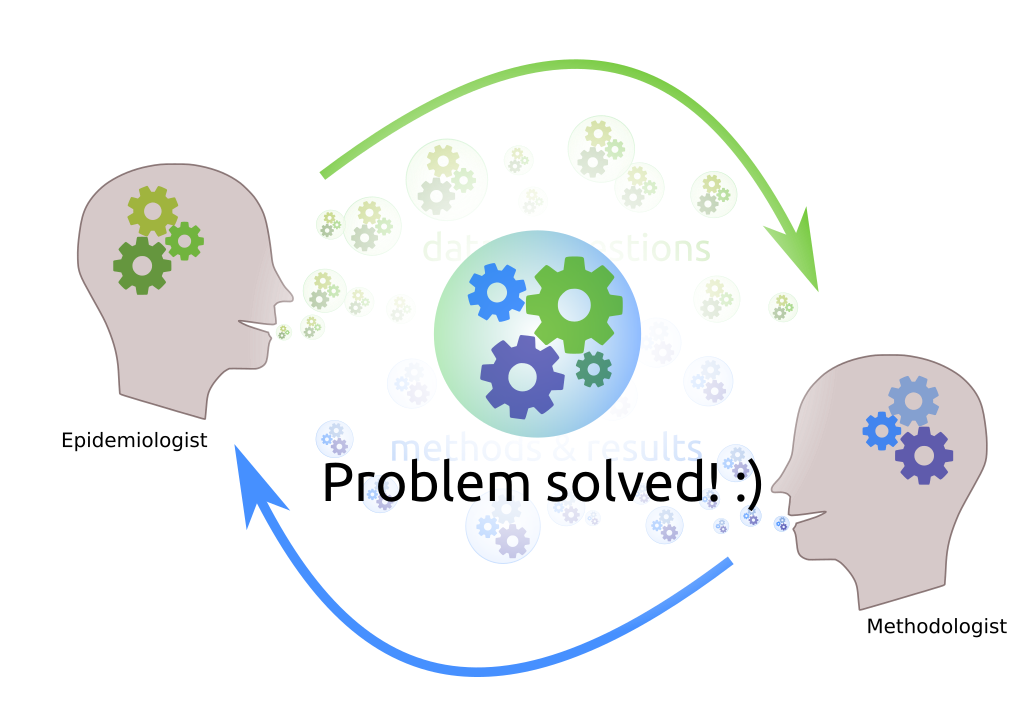
\includegraphics[width=.8\textwidth]{figs/dialogue5}}

\end{center}


\end{frame}
%%%%%%%%%%%%%%%%%%%%%%%%%%%%
%%%%%%%%%%%%%%%%%%%%%%%%%%%%






%%%%%%%%%%%%%%%%%%%%%%%%%%%%
%%%%%%%%%%%%%%%%%%%%%%%%%%%%
\begin{frame}[fragile]
  \frametitle{Outbreak response context creates distance and delays}

\begin{center} 

\only<1>{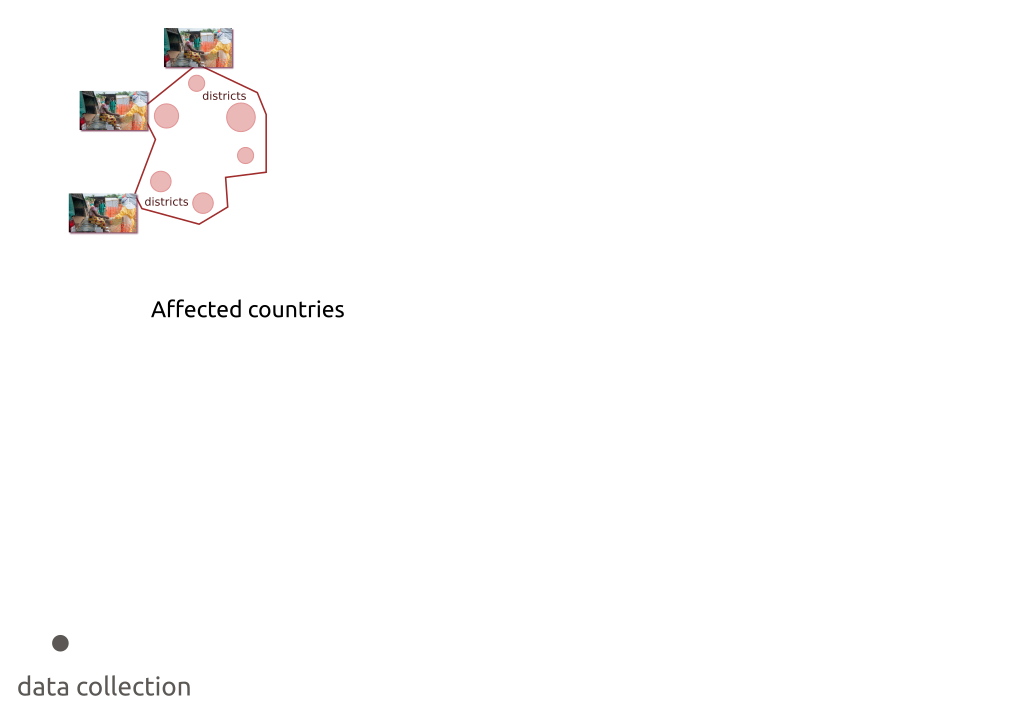
\includegraphics[width=.75\textwidth]{figs/process1}}\only<2>{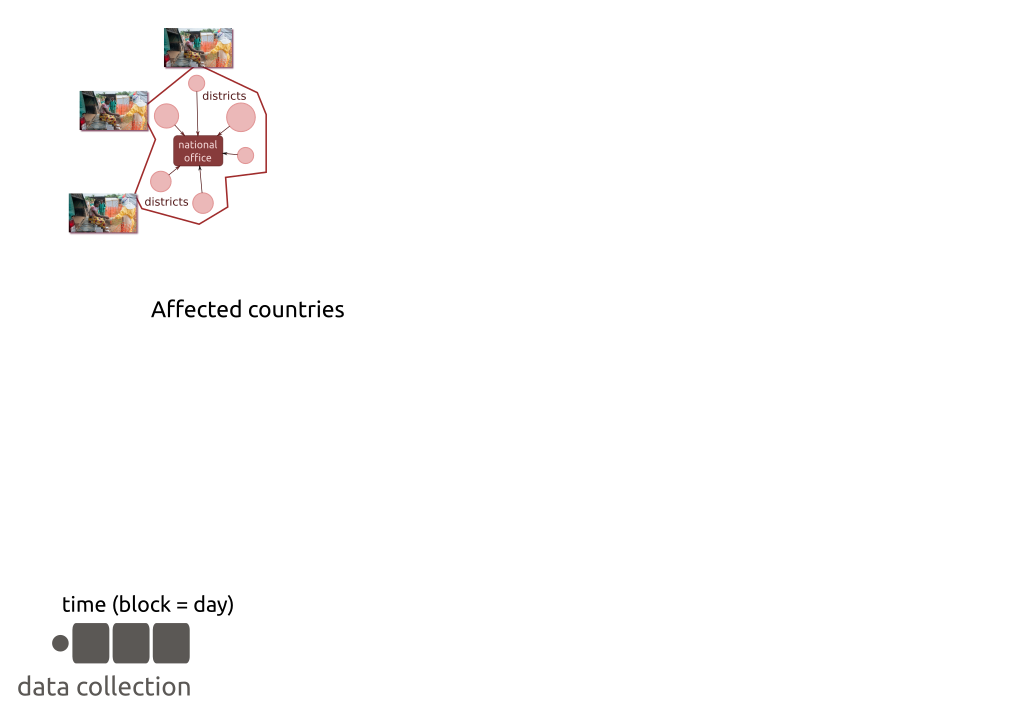
\includegraphics[width=.75\textwidth]{figs/process2}}\only<3>{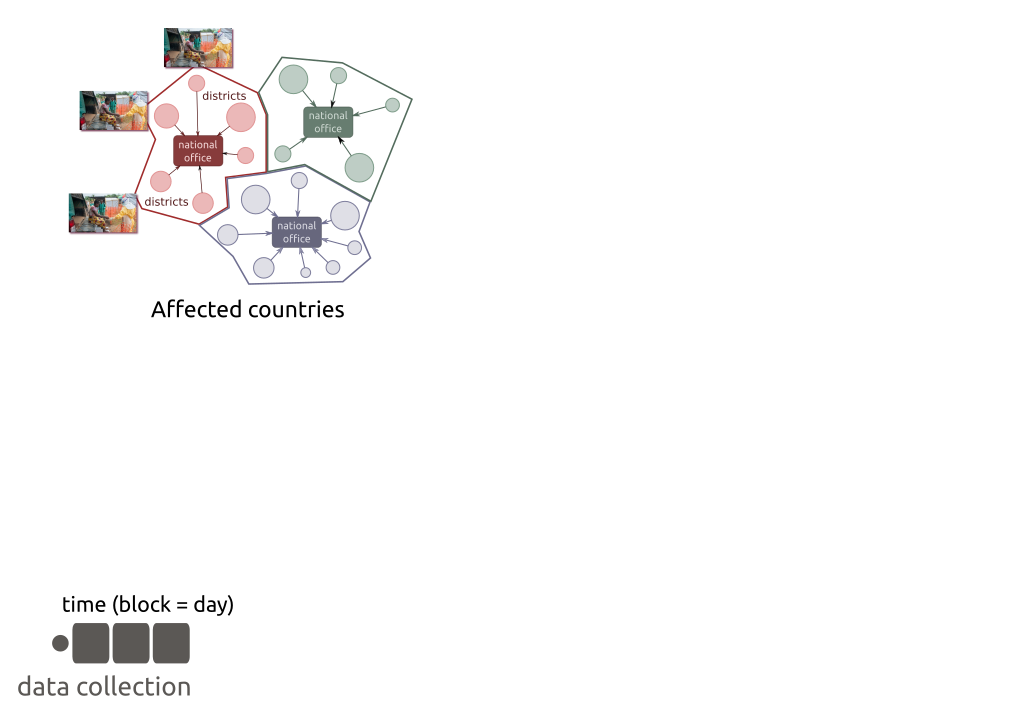
\includegraphics[width=.75\textwidth]{figs/process3}}\only<4>{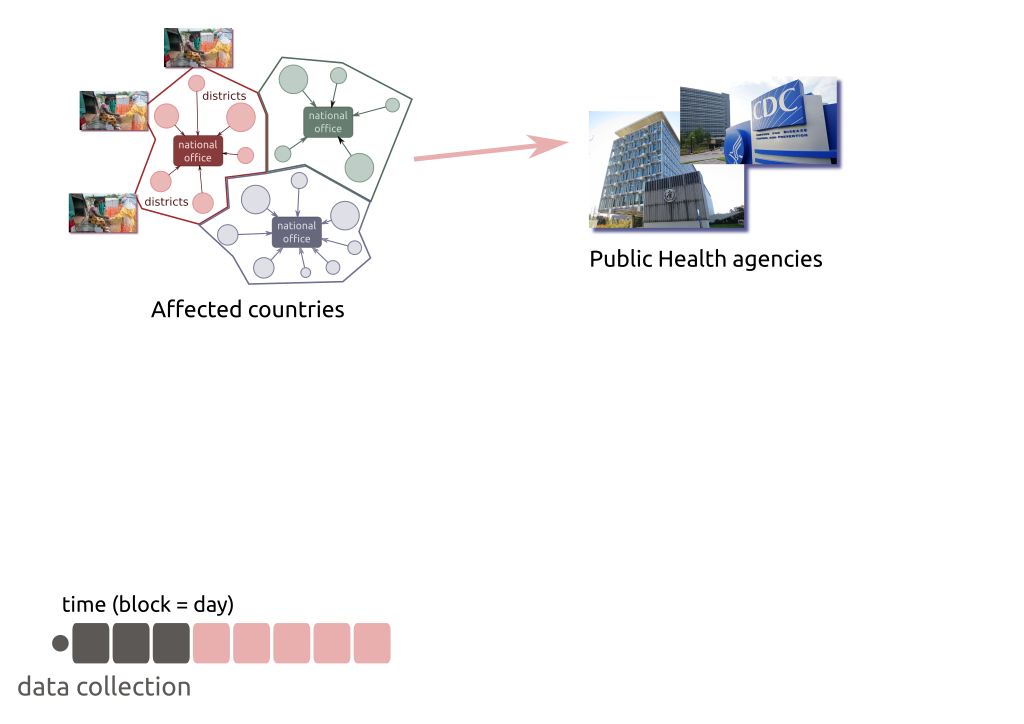
\includegraphics[width=.75\textwidth]{figs/process4}}\only<5>{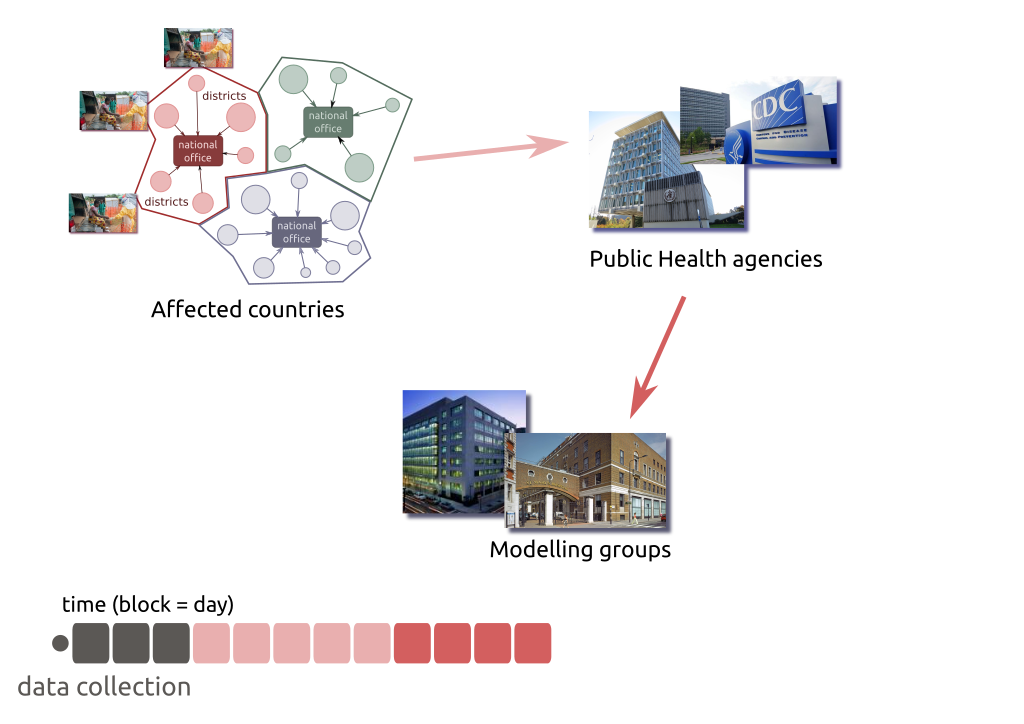
\includegraphics[width=.75\textwidth]{figs/process5}}\only<6>{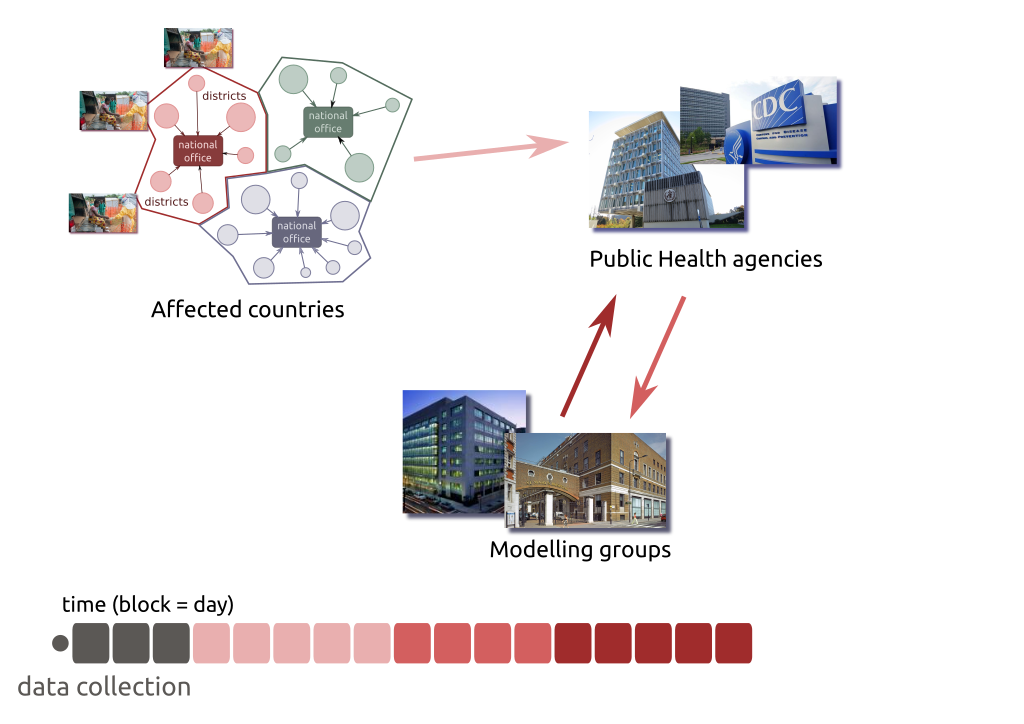
\includegraphics[width=.75\textwidth]{figs/process6}}\only<7->{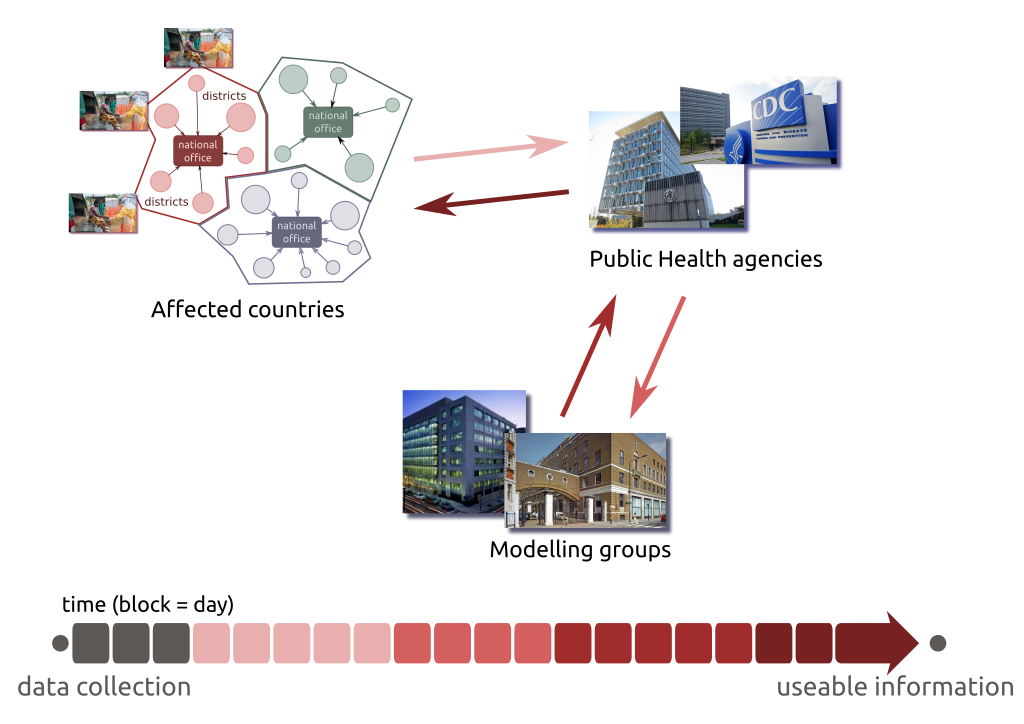
\includegraphics[width=.75\textwidth]{figs/process7}}

\begin{itemize}
\visible<8->{\item efficient tools can shorten delays}
\visible<9->{\item potential of \alert{embedding methodologists in outbreak response teams}}
\end{itemize}

\end{center}

\end{frame}
%%%%%%%%%%%%%%%%%%%%%%%%%%%%
%%%%%%%%%%%%%%%%%%%%%%%%%%%%





%%%%%%%%%%%%%%%%%%%%%%%%%%%%
%%%%%%%%%%%%%%%%%%%%%%%%%%%%
\begin{frame}[fragile]
  \frametitle{Thanks to...}

\begin{itemize}
\item \textbf{Mirna Panic}
\vspace{.3cm}
\item \textbf{Imperial College:} Neil Ferguson, Rich Fitzjohn, Anne Cori, Finlay Campbell, Evgenia Markvardt, James Hayward 
\vspace{.3cm}
\item \textbf{UC Berkeley:} Karthik Ram
\vspace{.3cm}
\item \textbf{Groups:} WHO Ebola Response Team, Hackout 1/2/3, RECON members, GOARN
\vspace{.3cm}
\item \textbf{funding:} HPRU-NIHR, MRC
\end{itemize}


\end{frame}
%%%%%%%%%%%%%%%%%%%%%%%%%%%%
%%%%%%%%%%%%%%%%%%%%%%%%%%%%





%%%%%%%%%%%%%%%%%%%%%%%%%%%%
%%%%%%%%%%%%%%%%%%%%%%%%%%%%
\begin{frame}[standout]
More on:\\
\emph{www.repidemicsconsortium.org}\\
~\\
Questions?
\end{frame}
%%%%%%%%%%%%%%%%%%%%%%%%%%%%
%%%%%%%%%%%%%%%%%%%%%%%%%%%%








\end{document}
